% GEM-PIC-RZ: manuscript draft
% Compile: pdflatex gempic_rz && pdflatex gempic_rz
\documentclass[aps,prab,reprint,floatfix,superscriptaddress,amsmath,amssymb]{revtex4-2}

\usepackage{graphicx}
\usepackage{bm}
\usepackage{booktabs}
\usepackage{tikz}
\usetikzlibrary{arrows.meta,decorations.pathmorphing}
\usepackage[colorlinks=true,linkcolor=blue,citecolor=blue,urlcolor=blue]{hyperref}

\newcommand{\dd}{\mathrm{d}}
\newcommand{\todo}[1]{\textcolor{red}{[#1]}}

\begin{document}

\title{GEM-PIC-RZ: a Galilean electromagnetic particle-in-cell code\\ in quasi-cylindrical geometry with free-hand grids}

\author{Alexander Pukhov}
\affiliation{Institut f\"ur Theoretische Physik I, Heinrich-Heine-Universit\"at D\"usseldorf, 40225 D\"usseldorf, Germany}

\date{\today}

\begin{abstract}
We present GEM-PIC-RZ, a particle-in-cell code for laser- and beam-driven plasma accelerators in quasi-cylindrical geometry (azimuthal Fourier modes). The code uses the Galilean variables $\zeta = z - ct$ and $s = ct$ of the GEM-PIC scheme. The electromagnetic field is split into its forward and backward characteristic components; the slow-time derivative is kept for the forward component, so the laser carrier is resolved on the $\zeta$ grid and evolves in $s$, while the backward and longitudinal components follow from integrals along $\zeta$. The resulting scheme has no Courant limit: the step in $s$ is set by diffraction and by the evolution of the plasma, not by the cell size, and can be thousands of laser wavelengths. The fields of a slice follow from two tridiagonal systems per azimuthal mode. The radial grid is staggered and non-uniform, with finite-volume operators that keep the discrete Gauss law exact, and the grids in $r$, $\zeta$ and $s$ are all free-hand: the step is given at reference points and interpolated in between. We derive the numerical dispersion relation, identify a stationary odd--even mode that causes numerical Cherenkov radiation behind relativistic bunches and remove it with a filter of the beam current. The code supports mobile ions, field ionization, particle bunches with their self-consistent initial fields at any energy, external transport elements, MPI pipelining along $\zeta$ combined with OpenMP threads, a GPU engine, and openPMD output on the native non-uniform grid. A laser wakefield benchmark against the full PIC code FBPIC agrees to 1.6\,\% in the on-axis wake at about 1/50 of the computing time. Because the carrier is resolved, the same equations also describe undulator radiation and free-electron lasers; this capability is summarized here and will be presented separately.
\end{abstract}

\maketitle

%---------------------------------------------------------------------------
\section{Introduction}\label{sec:intro}

Plasma-based accelerators driven by lasers~\cite{Tajima1979,Esarey2009} or particle beams are multiscale problems: the laser wavelength $\lambda_0 \sim 1\,\mu$m, the plasma wavelength $\lambda_p \sim 10$--$100\,\mu$m and the acceleration length of millimetres to metres. Full electromagnetic PIC codes resolve $\lambda_0$ and are limited by the Courant condition, so the number of time steps is the acceleration length divided by a fraction of $\lambda_0$. Quasi-cylindrical (azimuthal-mode) codes such as Calder-Circ and FBPIC~\cite{Lifschitz2009,Lehe2016} reduce the cost per step; the Lorentz-boosted frame~\cite{Vay2007} and Galilean coordinates with spectral solvers~\cite{Lehe2016b} reduce the number of steps or suppress the numerical Cherenkov instability, but the Courant limit remains.

Quasi-static codes~\cite{Sprangle1990,Mora1997,Lotov2003,Huang2006,Mehrling2014,Li2021,Diederichs2022,FerranPousa2019} remove it by dropping \emph{all} derivatives with respect to the slow time. The plasma response of a slice then follows from the sources of that slice, and the driver is advanced with a step set by its own evolution. The price is that the laser carrier can no longer be resolved: lasers enter through ponderomotive envelope models~\cite{Mora1997,Benedetti2018}, and radiation at the carrier frequency, harmonic generation, ionization in the instantaneous field and the emission of radiation by the beam are outside the model.

The GEM-PIC scheme~\cite{GEMPIC} occupies the space between the two. It writes Maxwell's equations in the Galilean variables $\zeta = z - ct$ and $s = ct$ and splits the field into its forward and backward characteristic components. The derivative with respect to the slow time $s$ is kept where it matters, for the forward component that carries the laser, so the carrier is resolved on the $\zeta$ grid and propagates, diffracts and is depleted and red-shifted self-consistently. It is dropped for the backward and longitudinal components, which then follow from ordinary differential equations along $\zeta$. The resulting scheme is \emph{not} a quasi-static approximation: the slow-time evolution of the radiation is retained. Yet, like quasi-static codes, it has no Courant limit, because the field update is implicit in the transverse operator.

This paper describes GEM-PIC-RZ, the implementation of the scheme in quasi-cylindrical geometry. Its main features are:
(i) the field equations of GEM-PIC for azimuthal modes $m = 0,\dots,M$, discretized on a staggered, non-uniform radial grid with finite-volume operators that make the discrete Gauss law exact and decouple the slice equations into two tridiagonal systems per mode (Secs.~\ref{sec:model}, \ref{sec:disc});
(ii) free-hand grids in $r$, $\zeta$ and $s$, which put resolution at the axis, at the laser pulse or a witness bunch, and in a density up-ramp (Sec.~\ref{sec:grids});
(iii) the numerical dispersion relation, which shows unconditional stability and a stationary $\zeta$-Nyquist mode, the source of a numerical Cherenkov radiation that a beam-current filter removes (Sec.~\ref{sec:dispersion});
(iv) a portable implementation with MPI pipelining along $\zeta$, OpenMP and GPU engines, checkpoints and openPMD output on the native grid (Sec.~\ref{sec:impl});
(v) a set of tests against analytic references and a benchmark against FBPIC (Sec.~\ref{sec:valid}).
Since the carrier is resolved, the same equations contain the spontaneous and stimulated emission of an electron beam in an undulator; Sec.~\ref{sec:fel} summarizes this free-electron-laser (FEL) capability, which will be the subject of a separate publication.

%---------------------------------------------------------------------------
\section{Model}\label{sec:model}

\subsection{Variables and field equations}

We use units with $c = 1$, lengths in $1/k_0$, time in $1/\omega_0$ ($k_0 = \omega_0/c$ the laser wavenumber), densities in the critical density $n_c$, momenta in $m_e c$ and fields in $m_e c\,\omega_0/e$. The co-moving coordinate and the slow time are
\begin{equation}
\zeta = z - t, \quad s = t; \qquad \partial_t = \partial_s - \partial_\zeta, \quad \partial_z = \partial_\zeta ,
\end{equation}
and the lab position is $z = \zeta + s$. The simulation window covers $0 \le \zeta \le L_w$; its front is at $\zeta = L_w$. Every field is expanded in azimuthal modes,
\begin{equation}
F(r,\varphi,\zeta,s) = F_0 + 2\,\mathrm{Re}\sum_{m=1}^{M} F_m(r,\zeta,s)\, e^{im\varphi},
\end{equation}
and we drop the mode index below. A linearly or circularly polarized laser lives in $m = 1$; $m = 0$ carries the wake.

The transverse fields are combined into the characteristic components
\begin{align}
R_r &= E_r + B_\varphi, & L_r &= E_r - B_\varphi, \nonumber\\
R_\varphi &= E_\varphi - B_r, & L_\varphi &= E_\varphi + B_r .
\end{align}
A wave travelling in $+z$ at the speed of light has $L = 0$ and is a function of $\zeta$ only; $R$ is the forward (laser) field. Maxwell's equations become, exactly,
\begin{align}
\partial_s R_r &= \partial_r E_z + \frac{im}{r} B_z - j_r, \label{eq:Rr}\\
\partial_s R_\varphi &= \frac{im}{r} E_z - \partial_r B_z - j_\varphi, \label{eq:Rp}\\
(\partial_s - 2\partial_\zeta) L_r &= -\Bigl(\partial_r E_z - \frac{im}{r}B_z + j_r\Bigr), \label{eq:Lr}\\
(\partial_s - 2\partial_\zeta) L_\varphi &= -\Bigl(\partial_r B_z + \frac{im}{r}E_z + j_\varphi\Bigr), \label{eq:Lp}\\
(\partial_s - \partial_\zeta) B_z &= -\frac{1}{r}\partial_r (r E_\varphi) + \frac{im}{r} E_r, \label{eq:Bz}\\
(\partial_s - \partial_\zeta) E_z &= \frac{1}{r}\partial_r (r B_\varphi) - \frac{im}{r} B_r - j_z . \label{eq:Ez}
\end{align}
The forward field varies fast in $\zeta$ (on $\lambda_0$) and slowly in $s$ (on the Rayleigh length and the depletion length). The backward field $L$ and the longitudinal fields $E_z$, $B_z$ of a co-propagating structure vary on the same $\zeta$ scales as their sources, which move with $v \approx c$, so their $s$-derivatives are small compared with their $\zeta$-derivatives. GEM-PIC-RZ keeps $\partial_s$ in Eqs.~\eqref{eq:Rr}, \eqref{eq:Rp} and drops it in Eqs.~\eqref{eq:Lr}--\eqref{eq:Ez}:
\begin{align}
\partial_\zeta L_r &= \tfrac12\Bigl(\partial_r E_z - \frac{im}{r}B_z + j_r\Bigr), \label{eq:Lr2}\\
\partial_\zeta L_\varphi &= \tfrac12\Bigl(\partial_r B_z + \frac{im}{r}E_z + j_\varphi\Bigr), \label{eq:Lp2}\\
\partial_\zeta B_z &= \frac{1}{r}\partial_r (r E_\varphi) - \frac{im}{r} E_r, \label{eq:Bz2}\\
\partial_\zeta E_z &= -\frac{1}{r}\partial_r (r B_\varphi) + \frac{im}{r} B_r + j_z , \label{eq:Ez2}
\end{align}
with $E = (R + L)/2$ and $B_\varphi = (R_r - L_r)/2$, $B_r = (L_\varphi - R_\varphi)/2$. Equations \eqref{eq:Lr2}--\eqref{eq:Ez2} are integrated from the front of the window, where $L = E_z = B_z = 0$, towards the rear. The model reproduces the paraxial wave equation for the laser, $\partial_s R \simeq (2\partial_\zeta)^{-1}\nabla_\perp^2 R$, with the full carrier, and the quasi-static wake equations in the limit $\partial_s R \to 0$. \todo{Check the ordering and its wording against the GEM-PIC paper~\cite{GEMPIC}; the equations above were written down from the implementation.}

\subsection{Particles}

Two kinds of macroparticles exist, both pushed with the relativistic Lorentz force in the fields reconstructed from the modes.

\emph{Streaming particles}: the plasma electrons, mobile ions and electrons freed by ionization. A fresh layer of plasma is loaded at the front of the window at every step $s^0 \to s^1 = s^0 + \Delta$, with the density $n(s^1)$ and a quiet start in $r^2$ and $\varphi$; one macroparticle represents the plasma of a ring of axial thickness $\Delta$. The layer then streams through the whole window, using $\zeta$ as the independent variable. In the time $\dd t$ a particle moves by $\dd\zeta = -(1 - v_z)\dd t$, so between two slices with the spacing $h_n$ it is pushed with
\begin{equation}
\dd t = \frac{h_n}{1 - v_z}, \label{eq:dt}
\end{equation}
by a two-pass Boris push~\cite{Boris1970} that makes $\dd t$ consistent with the mean $v_z$ over the interval. It deposits its current with the weight $W = q\,\dd t/\Delta$, the charge that crosses the cell during one step. The fields are those of the level $s^1$ being computed (Sec.~\ref{sec:march}).

\emph{Beam particles}: bunches and trapped particles, which move with the window. They are advanced in $s$ from $s^0$ to $s^1$ with the Vay pusher~\cite{Vay2008} in sub-steps of at most $\Delta z_\mathrm{max}$, in the fields of level $s^0$; the Vay pusher keeps the cancellation $\bm E + \bm v\times\bm B \approx 0$ of a relativistic beam in its own field at any step, which the Boris pusher does not. A beam particle deposits a current with the weight $q/v_z$, linear in $\zeta$.

The two lists exchange particles. A streaming particle whose lab position reaches $z = s^1$ inside the window has been trapped; it joins the beam list if $v_z \ge 0.9$. A slower one, which may happen in a strong laser field where electrons move forward by more than $\Delta$ while crossing the pulse, continues to stream in the next step from its $\zeta$. Conversely, a beam particle that becomes slower than $v_z = 0.8$ returns to streaming. No particle is deleted, so the charge is conserved.

\subsection{Initial fields}

A laser pulse is initialized in mode $m=1$ as a forward wave, $R_{r,1} = P^*$, $R_{\varphi,1} = iP^*$, $L = 0$, with $P = E_x + iE_y$ a paraxial Gaussian beam (with wavefront curvature and Gouy phase at a distance from focus) or a given radial profile.

A bunch of velocity $\beta$ starts with its own co-moving field, $-(\nabla_\perp^2 + \gamma^{-2}\partial_\zeta^2)\psi = j_z/\beta$, $R = (1 + \beta)\bm E_\perp$, $L = (1-\beta)\bm E_\perp$, $E_z = -\gamma^{-2}\partial_\zeta\psi$, with $\bm E_\perp = -\nabla_\perp\psi$. The problem is solved with the radial eigenvectors of the discrete Laplacian of the field solver and one tridiagonal solve along $\zeta$ per eigenvector, so a bunch in vacuum is an exact discrete equilibrium. A field that is not the co-moving one would stay behind a bunch with $v < c$ that slips back in the window and exchange energy with it; this matters for the FEL application (Sec.~\ref{sec:fel}). The radial wall and the ends of the window must not cut this field; the code prints the box size it needs ($r_\mathrm{max} \gtrsim \gamma\sigma_z$, gaps of a few $\gamma^{-1}r_\mathrm{max}$ at both ends).

\subsection{Ionization and ions}

Ion species can be mobile, with their own density profile (e.g.\ a dopant section), and field-ionizable. The ADK tunnel rate~\cite{ADK1986,Chen2013} of each level is evaluated with the instantaneous $|\bm E|$, including the laser carrier, and averaged over the two slices of the interval; ionization energies are taken from the NIST database~\cite{NIST}. A Monte Carlo step with exponential waiting times allows several levels per interval. The random numbers come from a counter-based hash of (seed, particle, step, slice, pass), so all back-ends draw the same numbers.

%---------------------------------------------------------------------------
\section{Discretization}\label{sec:disc}

\subsection{Radial grid and operators}

The radial grid has faces $\rho_i$, $i = 0,\dots,N$ ($\rho_0 = 0$ is the axis), and centres $c_i$, $i = 0,\dots,N-1$, $\rho_i < c_i < \rho_{i+1}$. Faces carry $R_r$, $L_r$, $B_z$, $j_r$; centres carry $R_\varphi$, $L_\varphi$, $E_z$, $j_\varphi$, $j_z$. With the finite-volume measures
\begin{equation}
A^f_i = \rho_i (c_i - c_{i-1}), \quad A^f_0 = \tfrac12 c_0^2, \qquad A^c_i = c_i(\rho_{i+1} - \rho_i),
\end{equation}
the operators are
\begin{align}
(G e)_i &= \frac{e_i - e_{i-1}}{c_i - c_{i-1}}, \qquad
(g b)_i = \frac{b_{i+1} - b_i}{\rho_{i+1} - \rho_i}, \\
(\mathrm{CE})_i &= \frac{c_i E_{\varphi,i} - c_{i-1}E_{\varphi,i-1}}{A^f_i} - \frac{im}{\rho_i}E_{r,i}, \\
(\mathrm{CB})_i &= \frac{\rho_{i+1}B_{\varphi,i+1} - \rho_i B_{\varphi,i}}{A^c_i} - \frac{im}{c_i}B_{r,i},
\end{align}
for $\partial_r$ to the faces and to the centres and for the two curls in Eqs.~\eqref{eq:Bz2}, \eqref{eq:Ez2}. Two discrete identities hold exactly on any grid,
\begin{equation}
\mathrm{CE}\bigl(G e,\ \tfrac{im}{c} e\bigr) = 0, \qquad \mathrm{CB}\bigl(\tfrac{im}{\rho} b,\ -g b\bigr) = 0, \label{eq:curlgrad}
\end{equation}
because $A^f_i = \rho_i(c_i - c_{i-1})$ and $A^c_i = c_i(\rho_{i+1}-\rho_i)$; they are the discrete forms of $\nabla\times\nabla = 0$ in the two staggerings. The divergence on the measures $A^c$ makes the discrete Gauss law exact. The particles deposit with area weighting plus a quadratic correction per interval, $w = x + \kappa x(1-x)$ with $x$ linear in $r^2$, where $\kappa$ is chosen so that the deposited volumes equal $A^f$, $A^c$: a uniform plasma is deposited exactly, also on a stretched grid. Fields are gathered linearly in $r$, which is exact near the axis for fields $\propto r$.

\subsection{The march in $\zeta$}\label{sec:march}

The window has slices $\zeta_0 = 0 < \zeta_1 < \dots < \zeta_{N_\zeta}$ with spacings $h_n = \zeta_{n+1} - \zeta_n$. Fields live on the slices, currents on the intervals (half-cells) between them. A step computes the level $s^1$ from $s^0$ by marching from the front slice to the rear. At slice $n$ the slice $n+1$ of level $s^1$ is known.

Equations~\eqref{eq:Rr}, \eqref{eq:Rp} are integrated with the trapezoidal rule in $s$,
\begin{equation}
R^1_n = R^0_n + \frac{\Delta}{2}\bigl[\mathcal F(E_z, B_z)^0_n + \mathcal F(E_z, B_z)^1_n\bigr] - \frac{\Delta}{4}\,\mathcal J_n, \label{eq:Rdisc}
\end{equation}
where $\mathcal F$ is the right-hand side without the current and $\mathcal J_n$ is the sum of the currents of the two adjacent half-cells at both levels. On a non-uniform $\zeta$ grid the current at the slice is the linear interpolation $(h_n j_{n-1/2} + h_{n-1} j_{n+1/2})/(h_{n-1} + h_n)$. Equations~\eqref{eq:Lr2}--\eqref{eq:Ez2} are integrated with the trapezoidal rule over the half-cell $h_n$, e.g.
\begin{equation}
L^1_n = L^1_{n+1} - \frac{h_n}{4}\bigl[\mathcal G^1_{n+1} + \mathcal G^1_n\bigr] - \frac{h_n}{2}\, j_{n+1/2}. \label{eq:Ldisc}
\end{equation}
$R^1_n$ and $L^1_n$ are linear in the unknown $E_z$ and $B_z$ of slice $n$. Inserted into the trapezoidal rules for Eqs.~\eqref{eq:Bz2}, \eqref{eq:Ez2}, the identities~\eqref{eq:curlgrad} remove $E_z$ from the $B_z$ equation and $B_z$ from the $E_z$ equation. What remains are two independent tridiagonal systems per mode,
\begin{align}
\bigl[16 - h_n(2\Delta + h_n)\,\nabla^2_{f,m}\bigr]\, B_{z,n} &= \text{known}, \\
\bigl[16 - h_n(2\Delta + h_n)\,\nabla^2_{c,m}\bigr]\, E_{z,n} &= \text{known} - 16 h_n\, j_{z,n+1/2},
\end{align}
with the discrete Laplacians on the faces and on the centres. $R$ and $L$ then follow explicitly. The matrices depend only on $m$, $\Delta$ and $h_n$; they are factorized once per distinct $h_n$ and recomputed only when $\Delta$ changes. The cost of a slice is linear in $N$ and $M$.

The currents of half-cell $n+\frac12$ at level $s^1$ depend on the fields of slice $n$, which are being computed. The march therefore uses a predictor--corrector: the predictor takes the fields of slice $n$ from the old level, $F^1_n \approx F^0_n$ (the slow evolution in $s$), the streaming particles are pushed through the half-cell and deposit, the slice is solved, and the push and solve are repeated with the new fields (two passes by default). When the half-cell is final, $R$ at slice $n+1$ is corrected for the difference between the predicted and the final current that entered its Eq.~\eqref{eq:Rdisc}.

Two closures complete the scheme. At the rear slice the half-cell behind the window is set equal to the last one (zero gradient); a zero current there would halve the source of $R$ and produce a growing spike. Near the outer radial boundary an optional absorber damps $R$.

\subsection{Numerical dispersion}\label{sec:dispersion}

For a single vacuum Fourier mode $\propto e^{ik_\zeta\zeta - i\omega s}$ with transverse wavenumber $k_\perp$ ($\nabla_\perp^2 \to -k_\perp^2$) on a uniform $\zeta$ grid, the scheme gives
\begin{equation}
\tan\frac{\omega\Delta}{2} = \frac{\Delta\, h\, k_\perp^2 \sin\theta}{16\sin^2(\theta/2) - h^2 k_\perp^2\cos^2(\theta/2)}, \qquad \theta = k_\zeta h. \label{eq:disp}
\end{equation}
$\omega$ is real for all $k_\zeta$, $k_\perp$, $\Delta$ and $h$: the scheme is unconditionally stable, with no Courant condition linking $\Delta$ to $h$ or to the radial cells. For $\theta \to 0$ and $\Delta \to 0$, $\omega \to 2k_\zeta k_\perp^2/(4k_\zeta^2 - k_\perp^2) \simeq k_\perp^2/(2k_\zeta)$, the paraxial diffraction of the exact $\omega = \sqrt{k_\zeta^2 + k_\perp^2} - k_\zeta$ in the Galilean frame. The step $\Delta$ is therefore limited by accuracy only: by the Rayleigh length of the laser, the plasma and betatron evolution, and in an undulator by the period (Sec.~\ref{sec:fel}).

Equation~\eqref{eq:disp} also shows a defect: at the $\zeta$-Nyquist wavenumber, $\theta = \pi$, $\omega = 0$ for every $k_\perp$. This odd--even mode is stationary in the window, like a relativistic bunch, so the macroparticle noise of the bunch current drives it resonantly; its group velocity $\dd\zeta/\dd s = -h^2k_\perp^2/8$ carries it slowly backwards. The result is a numerical Cherenkov radiation~\cite{Godfrey1974} behind the bunch, with $E_x = B_y$ (pure $R$) and a sign change from slice to slice. It does not act back coherently on the bunch, so it is radiation, not an instability, and it grows with the propagation distance and the shot noise; a smaller $\Delta$ does not help. A $(1,2,1)/4$ filter along $\zeta$ applied to the current of the beam particles, whose response $\cos^2(\theta/2)$ vanishes at $\theta = \pi$, removes the source. The plasma current is not filtered, so the wake is unchanged (Sec.~\ref{sec:cherenkov}).

\subsection{Free-hand grids}\label{sec:grids}

All three axes use the same mapping: the step $h(x)$ is given at reference points and is linear in between, and the nodes follow from $\dd x/\dd k = h(x)$ with $k$ the cell or step index. Within a segment the steps then grow geometrically and the nodes are analytic. The radial grid is fine at the axis and coarse outside; the $\zeta$ grid is fine at the laser pulse ($\gtrsim 20$ points per wavelength) or at a witness and coarse in between; the step in $s$ is small in a density up-ramp or in an undulator and large elsewhere. All slice equations above hold for any $h_n$, and the beam filter acts in index space, so it removes the odd--even mode at any local spacing. A uniform grid is the special case of a constant table and is reproduced bit for bit.

%---------------------------------------------------------------------------
\section{Implementation}\label{sec:impl}

GEM-PIC-RZ is written in C++17 without external dependencies apart from optional MPI and HDF5 libraries. The input is a structured deck with blocks for the grid, lasers, plasma, ion species, bunches, undulators and transport elements, output and numerics; all values carry physical units (or code units), and profiles of the plasma density, the laser, the bunch current and energy chirp and an undulator taper can be given as expressions, compiled once to a stack program. Unknown keys, wrong units and inconsistent settings are reported with file and line. Bunches can also be read from openPMD files of other codes, with resampling and the shot noise of the real electron number~\cite{Fawley2002}. External elements (quadrupoles, solenoids, active plasma lenses, thin chicanes as $R_{56}$ maps, planar and helical undulators) act on the particles only.

\paragraph*{Back-ends.} The serial step is the reference implementation. A parallel engine runs the same step as kernels written once as lambdas behind a thin portability layer; it compiles with a C++ compiler for OpenMP threads and with \texttt{nvcc} for NVIDIA GPUs. Fields, currents and particles stay in device memory for the whole run; per slice and pass there are three kernels (streaming push with deposition and ionization, field solve with one thread block per mode, slice preparation). The OpenMP engine reproduces the serial step bit for bit when both are compiled without FMA contraction, and an emulation of the GPU code paths on CPU threads (teams with barriers, atomic deposition, unordered appends) agrees with it to $10^{-9}$. \todo{GPU timings: the CUDA build compiles and its paths are tested in emulation; measurements on a GPU are pending.}

\paragraph*{MPI.} Within one step the march is sequential in $\zeta$, from the front to the rear. The window is therefore split into blocks of consecutive slices, one per rank, and the ranks form a pipeline in the steps: while rank $q$ computes step $k$, rank $q+1$, ahead of it in $\zeta$, already computes step $k+1$~\cite{Feng2009}. A rank passes to the rank behind it the boundary slice, the predicted current there, the streaming particles and the beam particles that drift across; the rank behind returns the corrected $R$ and ghost slices for the next step. The efficiency is $N_s/(N_s + P - 1)$ for $N_s$ steps and $P$ ranks, and the streaming plasma loads all slices equally. The ionization-injection example runs 1.90 times faster on two ranks than serially, as predicted, with identical results; the regression deck runs 1.8 times faster with two OpenMP threads. MPI combines with OpenMP threads on every rank; MPI results agree with the serial run to rounding, including runs with trapping and re-streaming of particles and restarts across rank counts.

\paragraph*{Output.} Rank 0 writes console diagnostics, bunch statistics (energy, spread, emittance, charge, also of the self-trapped charge), charge-state distributions, line-outs and maps, HDF5 files with all modes on the native grid, and checkpoints that hold the complete state including the random-number counters. A restart is exact, may change the step table in $s$, the output and the back-end, and may use any number of ranks. openPMD files~\cite{openPMD} hold the fields interpolated to a uniform $r$--$\zeta$ grid, readable by standard tools, and in addition the exact data on the native non-uniform nodes. openPMD~1.1 has no non-uniform meshes; the native records carry their node positions as data sets referenced by a mesh attribute \texttt{gridCoordinates}, the form we have proposed, together with the QUARZ code~\cite{QUARZ}, for the openPMD 2.0 standard~\cite{openPMDPR}.

\paragraph*{Tests.} A \texttt{ctest} suite of 23 tests runs in minutes: about 230 unit checks (parser, units, grids, deposition, atomic data, ADK rate), a regression deck for every back-end, the physics tests of Sec.~\ref{sec:valid}, MPI, restart, HDF5 and openPMD round trips.

%---------------------------------------------------------------------------
\section{Tests and benchmarks}\label{sec:valid}

\subsection{Verification}

Table~\ref{tab:tests} lists the tests against analytic or independent references.

\begin{table}[htb]
\caption{Verification tests (all in the test suite).}\label{tab:tests}
\begin{ruledtabular}
\begin{tabular}{p{0.52\columnwidth}p{0.4\columnwidth}}
test & result \\ \hline
Field of an ultra-relativistic bunch in vacuum vs Gauss's law (uniform, stretched and free-hand radial grids) & $E_r$ to $5\times10^{-4}$; noise $E_z < 2\times10^{-3}E_r$ \\
Same on a free-hand $\zeta$ grid (2.5--8\,$k_0^{-1}$ across the bunch) & $2\times10^{-3}$ (shot-noise level) \\
$\gamma = 100$ bunch in its own field, 8\,cm & energy kept to $2\times10^{-5}$ \\
Laser focusing in vacuum ($w_0 = 5\,\mu$m, $z_R = 98\,\mu$m, 0.4\,mm) & $a_0(z)$ within 3\,\% \\
Ion collapse in a dense bunch ($n_b = 100 n_0$, H)~\cite{Rosenzweig2005} vs test-ion model & on-axis $n_i$ 1--3\,\%; D/H delay 1.418 ($\sqrt2$) \\
Field ionization of H vs $1 - \exp(-\int w\,\dd t)$ & 0.02294 vs 0.02288 \\
N$^{5+}\to$N$^{6+}\to$N$^{7+}$ ($a_0 = 2.2$) vs rate equations & 0.9357/0.0600/0.0044 vs 0.9367/0.0593/0.0041 \\
ADK rate vs Landau rate (H-like ions) & $10^{-12}$ \\
Immobile limit of ions ($M = 10^{15}$\,u) & identical fields \\
\end{tabular}
\end{ruledtabular}
\end{table}

\subsection{Free-hand $\zeta$ and $s$ grids}

A beam-driven wake in a plasma of $0.002\,n_c$, with a driver of $\sigma_z = 1.5\,k_0^{-1}$ and a witness $130\,k_0^{-1}$ behind, was run on three $\zeta$ grids (Table~\ref{tab:zgrid}). A uniform coarse grid ($h = 2$) is 16\,\% off at the driver; a free-hand grid that is fine ($h = 0.25$) only at the two bunches reproduces the fine uniform grid to $10^{-3}$ with a quarter of the slices and 3.6 times faster. In the laser wakefield example, a free-hand step in $s$ that is small only in the density up-ramp gives the witness energy within 0.4\,\% of a run with uniformly small steps, with 44 instead of 80 steps; uniform large steps are 1.4\,\% off.

\begin{table}[htb]
\caption{Beam-driven wake on uniform and free-hand $\zeta$ grids. $E_z$ errors relative to $\max|E_z|$, witness energy change over 50 steps.}\label{tab:zgrid}
\begin{ruledtabular}
\begin{tabular}{lccc}
$\zeta$ grid & slices & $E_z$ error\footnotemark[1] & $\Delta E$ error \\ \hline
uniform $h = 0.25$ (ref.) & 2800 & -- & -- \\
uniform $h = 2$ & 350 & 16\,\% / 6.6\,\% & 1.3\,\% \\
free-hand 0.25 / 2 & 734 & 0.11\,\% / 0.84\,\% & 0.06\,\% \\
\end{tabular}
\footnotetext[1]{At the driver / at the witness.}
\end{ruledtabular}
\end{table}

\subsection{Numerical Cherenkov radiation}\label{sec:cherenkov}

A bunch of 1\,pC at $\gamma = 1000$ ($\sigma_r = 2$, $\sigma_z = 4\,k_0^{-1}$, 16 slices) propagates 1000 steps of $\Delta = 20\,k_0^{-1}$ in vacuum. Without the filter the $\zeta$-Nyquist part of the field energy grows to $8.6\times10^{-2}$ of the total; with the filter it stays at $1.3\times10^{-4}$, the floor of the estimator. In a plasma wake ($0.002\,n_c$, 0.2\,pC driver) the Nyquist fraction grows from $1.3$ to $1.9\times10^{-2}$ between 200 and 400 steps without the filter and stays at $8\times10^{-5}$ with it, while the bunch parameters agree to four digits and the wake to 0.35\,\%. The filter damps structure on a scale of 31 cells per wavelength by 1\,\% per pass; bunches with structure of a few cells are under-resolved anyway.

\subsection{Laser wakefield: comparison with FBPIC}\label{sec:fbpic}

\begin{figure}[htb]
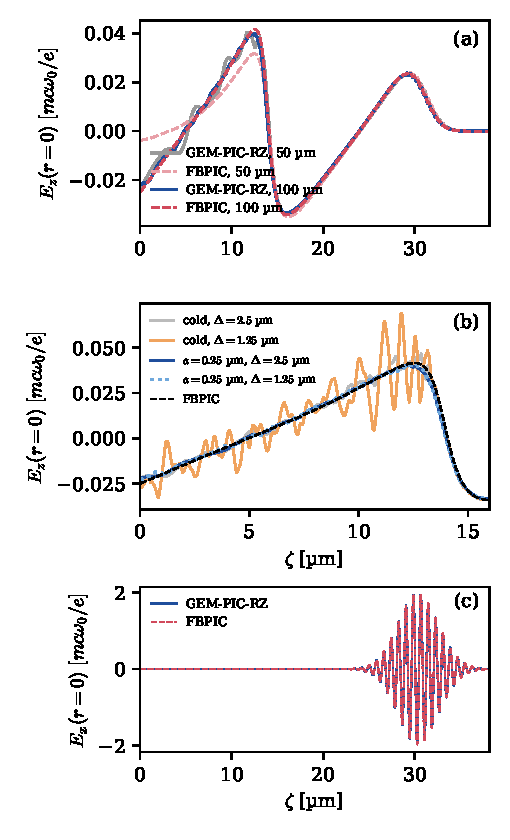
\includegraphics[width=\columnwidth]{figs/fig_lwfa.pdf}
\caption{Laser wakefield benchmark: (a) on-axis $E_z$ after 50 and 100\,$\mu$m of propagation, GEM-PIC-RZ (solid) and FBPIC (dashed); (b) the laser field $E_x$ on the axis at 100\,$\mu$m. The laser moves to the right.}\label{fig:lwfa}
\end{figure}

We compare with the quasi-cylindrical spectral full PIC code FBPIC~\cite{Lehe2016}. A laser of $\lambda_0 = 0.8\,\mu$m, $a_0 = 2$, $w_0 = 8.02\,\mu$m and a field duration of 10.6\,fs (1/e half length 3.18\,$\mu$m), linearly polarized and starting at focus, enters a plasma of $n_0 = 3.48\times10^{18}$\,cm$^{-3}$ ($0.002\,n_c$) after a 20\,$\mu$m linear ramp; the plasma column has a radius of 19.1\,$\mu$m and the ions are immobile. FBPIC uses $\Delta z = \lambda_0/32$, $\Delta r = 0.2\,\mu$m, two modes and 16 particles per cell. Figure~\ref{fig:lwfa} shows the on-axis fields. After 100\,$\mu$m the first wake period agrees to 1.6\,\% rms of the peak field, the minimum of $E_z$ is $-0.0339$ vs $-0.0342\,m_ec\omega_0/e$, and the laser peak field 1.971 vs 1.954. Further back, where the wave has steepened close to breaking, both codes show the same spiky structure. At 50\,$\mu$m the rear of the window is still in the up-ramp in FBPIC, so its wake is weaker there: GEM-PIC-RZ loads the plasma of a step at the front of the window with the density $n(s)$ of that step, so the profile is a function of the propagation distance and constant across the window. This difference matters only where the density changes over a window length. On one CPU core GEM-PIC-RZ took 1.7\,min, FBPIC about 1.5\,h.

\todo{Further benchmarks planned: beam-driven blowout against a quasi-static code (LCODE / QPAD / HiPACE++); laser depletion and red-shift over several Rayleigh lengths against FBPIC; ionization injection against FBPIC.}

%---------------------------------------------------------------------------
\section{Undulator radiation and free-electron lasers}\label{sec:fel}

Because the carrier is resolved in $\zeta$ and the forward field evolves in $s$, a beam that wiggles in a static undulator field radiates through the transverse current in Eqs.~\eqref{eq:Rr}, \eqref{eq:Rp}, and the radiation acts back on the beam through the gather; the radiation stays at fixed $\zeta$ while the electrons slip back by $\lambda_r$ per period. Spontaneous and coherent emission and the FEL interaction are therefore contained in the same equations, with the full space-charge fields of the beam and without the period averaging and slice approximations of dedicated FEL codes~\cite{Reiche1999}. The $\zeta$ grid resolves $\lambda_r$ ($\lambda_r/16$ or finer), the step in $s$ the undulator period ($\lambda_u/16$). Two details of the beam push were needed for a correct FEL coupling at such steps: the undulator field is averaged exactly over the step [a factor $\mathrm{sinc}(k_u\Delta z/2)$], and the current is deposited with the velocity at the time of the position, not half a sub-step earlier.

In brief: the coherent spontaneous emission of a short bunch in a planar undulator agrees with the far-field radiation integral to 2--4\,\% in energy (converging to $-2$\,\% with $\Delta\zeta$) and to $2\times10^{-4}$ in the spectral peak; the SASE gain length of a compact FEL agrees with the Ming Xie fit~\cite{Xie1995} (6.3 vs 6.4 periods); and seeded amplifiers at 10\,nm and 0.8\,nm agree with GENESIS~1.3~\cite{Reiche1999} to 4\,\% and 0.6\,\% in gain length when GENESIS includes the space-charge effects that GEM-PIC-RZ contains by construction. A combined simulation of plasma acceleration, beam transport and FEL amplification in one code, and the details of these tests, will be presented in a separate publication.

%---------------------------------------------------------------------------
\section{Discussion and conclusions}\label{sec:concl}

GEM-PIC-RZ solves Maxwell's equations in the Galilean variables $(\zeta, s)$ with the slow-time derivative kept for the forward field. It resolves the laser carrier, as a full PIC code, and has no Courant limit, as a quasi-static code. Its step in $s$ is set by the physics: hundreds to thousands of $k_0^{-1}$ in a plasma accelerator, a fraction of the period in an undulator. The discretization on staggered, non-uniform radial nodes keeps the discrete Gauss law and $\nabla\times\nabla = 0$ exact and reduces each slice to two tridiagonal systems per mode; free-hand grids in all three directions put the resolution where it is needed. The dispersion analysis exposes a stationary $\zeta$-Nyquist mode, and a filter of the beam current removes the numerical Cherenkov radiation it would cause, without touching the plasma response.

The model's limits follow from its ordering. Backward-propagating radiation (Raman backscatter, reflection from overdense plasma) is not described, since $\partial_s L$ is dropped, and the plasma density is sampled per step at the front of the window. Within these limits the code agrees with a full PIC code at a small fraction of its cost, and it extends naturally to radiation by the accelerated beam. Planned work includes cross-code benchmarks for beam-driven wakes and for laser depletion, GPU performance measurements, and the FEL applications.

GEM-PIC-RZ is open source~\cite{GEMPICRZ}; the decks and scripts of the tests in this paper are part of the repository.

\todo{Optional: a paragraph on the development of the code with an AI agent, as in the QUARZ paper~\cite{QUARZ}, if wanted.}

\begin{acknowledgments}
\todo{Funding, computing time.}
\end{acknowledgments}

\begin{thebibliography}{99}
\bibitem{Tajima1979} T. Tajima and J. M. Dawson, Laser electron accelerator, Phys. Rev. Lett. \textbf{43}, 267 (1979).
\bibitem{Esarey2009} E. Esarey, C. B. Schroeder, and W. P. Leemans, Physics of laser-driven plasma-based electron accelerators, Rev. Mod. Phys. \textbf{81}, 1229 (2009).
\bibitem{Lifschitz2009} A. F. Lifschitz \textit{et al.}, Particle-in-cell modelling of laser--plasma interaction using Fourier decomposition, J. Comput. Phys. \textbf{228}, 1803 (2009).
\bibitem{Lehe2016} R. Lehe, M. Kirchen, I. A. Andriyash, B. B. Godfrey, and J.-L. Vay, A spectral, quasi-cylindrical and dispersion-free particle-in-cell algorithm, Comput. Phys. Commun. \textbf{203}, 66 (2016).
\bibitem{Vay2007} J.-L. Vay, Noninvariance of space- and time-scale ranges under a Lorentz transformation and the implications for the study of relativistic interactions, Phys. Rev. Lett. \textbf{98}, 130405 (2007).
\bibitem{Lehe2016b} R. Lehe, M. Kirchen, B. B. Godfrey, A. R. Maier, and J.-L. Vay, Elimination of numerical Cherenkov instability in flowing-plasma particle-in-cell simulations by using Galilean coordinates, Phys. Rev. E \textbf{94}, 053305 (2016).
\bibitem{Sprangle1990} P. Sprangle, E. Esarey, and A. Ting, Nonlinear theory of intense laser-plasma interactions, Phys. Rev. Lett. \textbf{64}, 2011 (1990).
\bibitem{Mora1997} P. Mora and T. M. Antonsen, Jr., Kinetic modeling of intense, short laser pulses propagating in tenuous plasmas, Phys. Plasmas \textbf{4}, 217 (1997).
\bibitem{Lotov2003} K. V. Lotov, Fine wakefield structure in the blowout regime of plasma wakefield accelerators, Phys. Rev. ST Accel. Beams \textbf{6}, 061301 (2003).
\bibitem{Huang2006} C. Huang \textit{et al.}, QUICKPIC: A highly efficient particle-in-cell code for modeling wakefield acceleration in plasmas, J. Comput. Phys. \textbf{217}, 658 (2006).
\bibitem{Mehrling2014} T. Mehrling \textit{et al.}, HiPACE: a quasi-static particle-in-cell code, Plasma Phys. Control. Fusion \textbf{56}, 084012 (2014).
\bibitem{Li2021} F. Li \textit{et al.}, A quasi-static particle-in-cell algorithm based on an azimuthal Fourier decomposition for highly efficient simulations of plasma-based acceleration: QPAD, Comput. Phys. Commun. \textbf{261}, 107784 (2021).
\bibitem{Diederichs2022} S. Diederichs \textit{et al.}, HiPACE++: A portable, 3D quasi-static particle-in-cell code, Comput. Phys. Commun. \textbf{278}, 108421 (2022).
\bibitem{FerranPousa2019} A. Ferran Pousa, R. Assmann, and A. Martinez de la Ossa, Wake-T: a fast particle tracking code for plasma-based accelerators, J. Phys.: Conf. Ser. \textbf{1350}, 012056 (2019).
\bibitem{Benedetti2018} C. Benedetti, C. B. Schroeder, C. G. R. Geddes, E. Esarey, and W. P. Leemans, An accurate and efficient laser-envelope solver for the modeling of laser-plasma accelerators, Plasma Phys. Control. Fusion \textbf{60}, 014002 (2018).
\bibitem{GEMPIC} A. Pukhov, GEM-PIC: \todo{title, journal (J. Comput. Phys., submitted / in press)} (2026).
\bibitem{Boris1970} J. P. Boris, Relativistic plasma simulation -- optimization of a hybrid code, in \textit{Proc. 4th Conf. Numer. Simul. Plasmas} (Naval Research Laboratory, Washington, DC, 1970), p.~3.
\bibitem{Vay2008} J.-L. Vay, Simulation of beams or plasmas crossing at relativistic velocity, Phys. Plasmas \textbf{15}, 056701 (2008).
\bibitem{ADK1986} M. V. Ammosov, N. B. Delone, and V. P. Krainov, Tunnel ionization of complex atoms and of atomic ions in an alternating electromagnetic field, Sov. Phys. JETP \textbf{64}, 1191 (1986).
\bibitem{Chen2013} M. Chen, E. Cormier-Michel, C. G. R. Geddes, D. L. Bruhwiler, L. L. Yu, E. Esarey, C. B. Schroeder, and W. P. Leemans, Numerical modeling of laser tunneling ionization in explicit particle-in-cell codes, J. Comput. Phys. \textbf{236}, 220 (2013).
\bibitem{NIST} A. Kramida, Yu. Ralchenko, J. Reader, and NIST ASD Team, NIST Atomic Spectra Database (ver. 5.12), \url{https://physics.nist.gov/asd} (2026).
\bibitem{Godfrey1974} B. B. Godfrey, Numerical Cherenkov instabilities in electromagnetic particle codes, J. Comput. Phys. \textbf{15}, 504 (1974).
\bibitem{Fawley2002} W. M. Fawley, Algorithm for loading shot noise microbunching in multidimensional, free-electron laser simulation codes, Phys. Rev. ST Accel. Beams \textbf{5}, 070701 (2002).
\bibitem{Feng2009} B. Feng \textit{et al.}, Enhancing parallel quasi-static particle-in-cell simulations with a pipelining algorithm, J. Comput. Phys. \textbf{228}, 5340 (2009).
\bibitem{openPMD} A. Huebl \textit{et al.}, openPMD: A meta data standard for particle and mesh based data, \href{https://doi.org/10.5281/zenodo.591699}{doi:10.5281/zenodo.591699} (2015).
\bibitem{openPMDPR} Rectilinear meshes, pull request \#299 to the openPMD standard (branch upcoming-2.0.0), \url{https://github.com/openPMD/openPMD-standard/pull/299} (2026).
\bibitem{QUARZ} A. Pukhov and T. C. Wilson, QUARZ: a quasi-static particle-in-cell code with non-uniform radial grids for plasma wakefields, arXiv:2610.16910 (2026).
\bibitem{Rosenzweig2005} J. B. Rosenzweig \textit{et al.}, Effects of ion motion in intense beam-driven plasma wakefield accelerators, Phys. Rev. Lett. \textbf{95}, 195002 (2005).
\bibitem{Reiche1999} S. Reiche, GENESIS 1.3: a fully 3D time-dependent FEL simulation code, Nucl. Instrum. Methods Phys. Res., Sect. A \textbf{429}, 243 (1999).
\bibitem{Xie1995} M. Xie, Design optimization for an X-ray free electron laser driven by SLAC linac, in \textit{Proc. PAC'95} (IEEE, 1995), p.~183.
\bibitem{GEMPICRZ} A. Pukhov, GEM-PIC-RZ, \url{https://github.com/AlexMPukhov/GEM-PIC-RZ} (2026).
\end{thebibliography}

\end{document}
